\documentclass[aspectratio=169]{../latex_main/tntbeamer}  % you can pass all options of the beamer class, e.g., 'handout' or 'aspectratio=43'
\usepackage{dsfont}
\usepackage{bm}
\usepackage[english]{babel}
\usepackage[T1]{fontenc}
%\usepackage[utf8]{inputenc}
\usepackage{graphicx}
\graphicspath{ {./figures/} }
\usepackage{algorithm}
\usepackage[ruled,vlined,algo2e,linesnumbered]{algorithm2e}
\usepackage{hyperref}
\usepackage{booktabs}
\usepackage{mathtools}

\usepackage{amsmath,amssymb}

\DeclareMathOperator*{\argmax}{arg\,max}
\DeclareMathOperator*{\argmin}{arg\,min}

\usepackage{pgfplots}
\pgfplotsset{compat=1.16}
\usepackage{tikz}
\usetikzlibrary{trees} 
\usetikzlibrary{shapes.geometric}
\usetikzlibrary{positioning,shapes,shadows,arrows,calc,mindmap}
\usetikzlibrary{positioning,fadings,through}
\usetikzlibrary{decorations.pathreplacing}
\usetikzlibrary{intersections}
\pgfdeclarelayer{background}
\pgfdeclarelayer{foreground}
\pgfsetlayers{background,main,foreground}
\tikzstyle{activity}=[rectangle, draw=black, rounded corners, text centered, text width=8em]
\tikzstyle{data}=[rectangle, draw=black, text centered, text width=8em]
\tikzstyle{myarrow}=[->, thick, draw=black]

% Define the layers to draw the diagram
\pgfdeclarelayer{background}
\pgfdeclarelayer{foreground}
\pgfsetlayers{background,main,foreground}

% Requires XeLaTeX or LuaLaTeX
\usepackage{unicode-math}

\usepackage{fontspec}
%\setsansfont{Arial}
\setsansfont{RotisSansSerifStd}[ 
Path=../latex_main/fonts/,
Extension = .otf,
UprightFont = *-Regular,  % or *-Light
BoldFont = *-ExtraBold,  % or *-Bold
ItalicFont = *-Italic
]
\setmonofont{Cascadia Mono}[
Scale=0.8
]

% scale factor adapted; mathrm font added (Benjamin Spitschan @TNT, 2021-06-01)
%\setmathfont[Scale=1.05]{Libertinus Math}
%\setmathrm[Scale=1.05]{Libertinus Math}

% other available math fonts are (not exhaustive)
% Latin Modern Math
% XITS Math
% Libertinus Math
% Asana Math
% Fira Math
% TeX Gyre Pagella Math
% TeX Gyre Bonum Math
% TeX Gyre Schola Math
% TeX Gyre Termes Math

% Literature References
\newcommand{\lit}[2]{\href{#2}{\footnotesize\color{black!60}[#1]}}

%%% Beamer Customization
%----------------------------------------------------------------------
% (Don't) Show sections in frame header. Options: 'sections', 'sections light', empty
\setbeamertemplate{headline}{empty}

% Add header logo for normal frames
\setheaderimage{
	% 
\includegraphics[height=\logoheight]{figures/TNT_darkv4.pdf}
	
\includegraphics[height=\logoheight]{../latex_main/figures/luh_logo_rgb_0_80_155.pdf}
	% 
\includegraphics[height=\logoheight]{figures/logo_tntluh.pdf}
}

% Header logo for title page
\settitleheaderimage{
	% 
\includegraphics[height=\logoheight]{figures/TNT_darkv4.pdf}
	
\includegraphics[height=\logoheight]{../latex_main/figures/luh_logo_rgb_0_80_155.pdf}
	% 
\includegraphics[height=\logoheight]{figures/logo_tntluh.pdf}
}

% Title page: tntdefault 
\setbeamertemplate{title page}[tntdefault]  % or luhstyle
% Add optional title image here
%\addtitlepageimagedefault{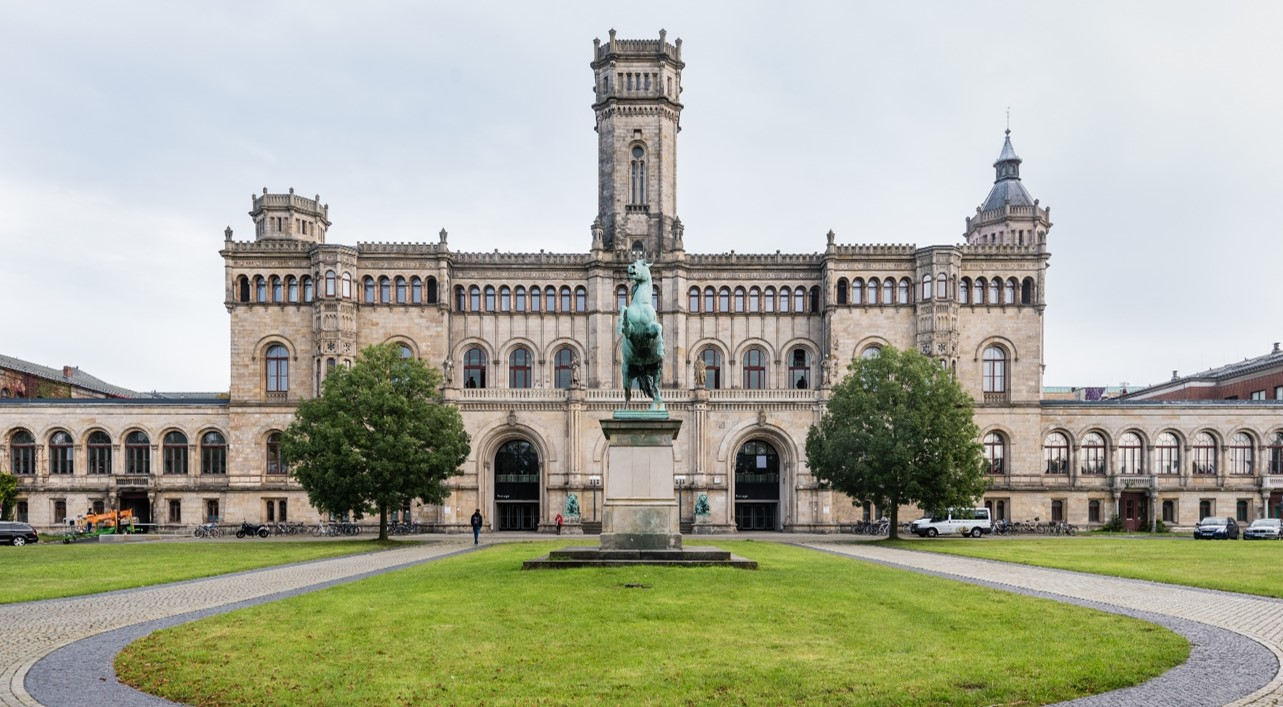
\includegraphics[width=0.65\textwidth]{figures/luh_default_presentation_title_image.jpg}}

% Title page: luhstyle
% \setbeamertemplate{title page}[luhstyle]
% % Add optional title image here
% \addtitlepageimage{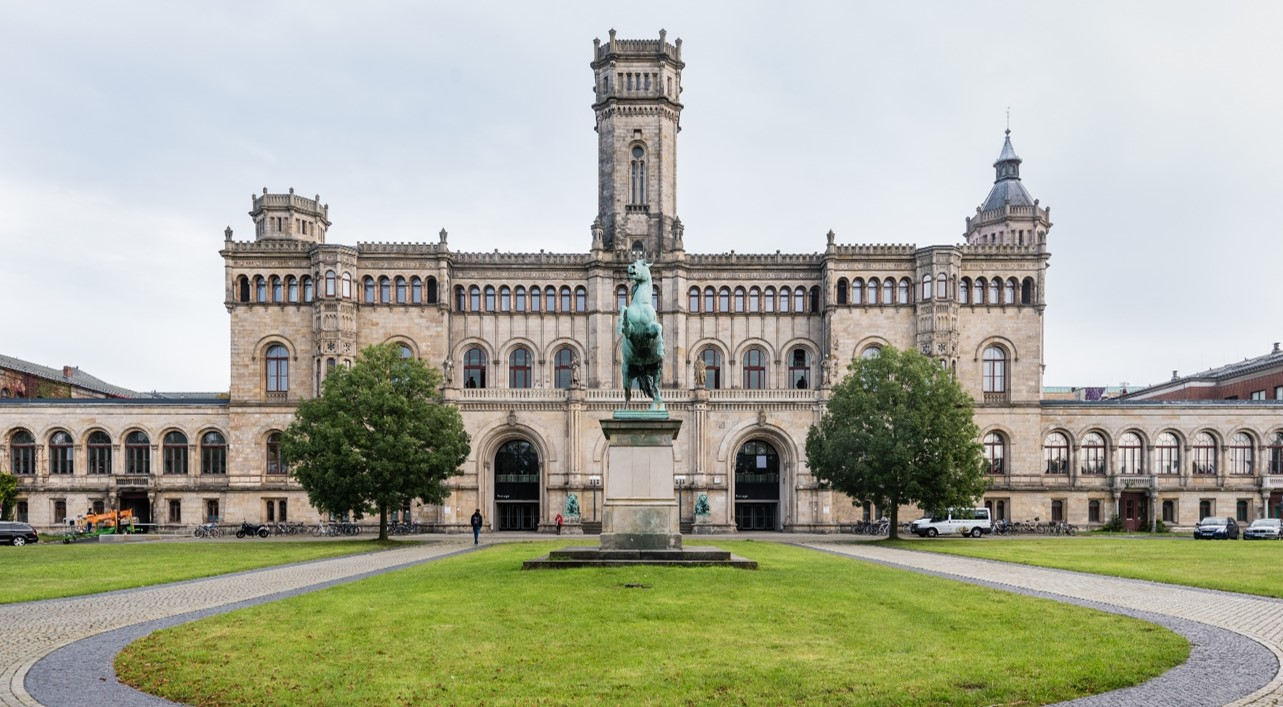
\includegraphics[width=0.75\textwidth]{figures/luh_default_presentation_title_image.jpg}}

\author[Lindauer \& Anand]{Marius Lindauer and Avishek Anand\\[1em]
	
\includegraphics[height=\logoheight]{../latex_main/figures/luh_logo_rgb_0_80_155.pdf}\qquad

\includegraphics[height=\logoheight]{../latex_main/figures/TNT_darkv4}\qquad

\includegraphics[height=\logoheight]{../latex_main/figures/L3S.jpg}	}
\date{Winter Term 2021
}


%%% Custom Packages
%----------------------------------------------------------------------
% Create dummy content
\usepackage{blindtext}

% Adds a frame with the current page layout. Just call \layout inside of a frame.
\usepackage{layout}


\title[Introduction]{iML: Interpretable Models}
\subtitle{Exemplary Applications}

%\institute{}


\begin{document}
	
	\maketitle

	%-----------------------------------------------------------------------------------------------------------------------------

    \begin{frame}{Bike Rentals (Regression)}
        
        \begin{itemize}
            \item Target: number of rented bikes
            \item Source: bicycle rental company Capital-Bikeshare in Washington D.C.,
            \item Reference: \lit{Fanaee-T and Gama. 2014}{https://link.springer.com/article/10.1007/s13748-013-0040-3}
            \item Exemplary features:
            \begin{itemize}
                \item season: spring, summer, fall or winter.
                \item holiday or not.
                \item working day or weekend
                \item weather situation on that day 
                \item temperature
            \end{itemize}
        \end{itemize}
        
    \end{frame}
    
    \begin{frame}{Regression on Bike Rentals}
        
        \centering
        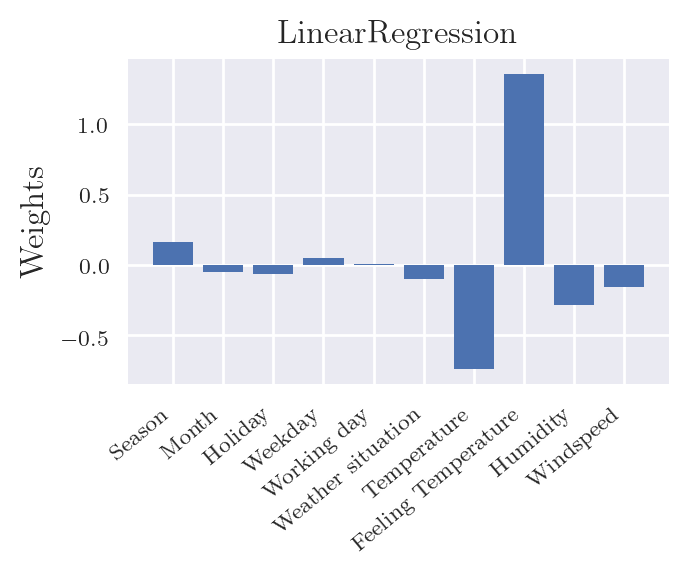
\includegraphics[width=0.55\textwidth]{w02_interpretable_models/figures/lin_bikesharing.png}

    \end{frame}
    
    \begin{frame}{Decision Tree on Bike Rentals}
        
        \centering
        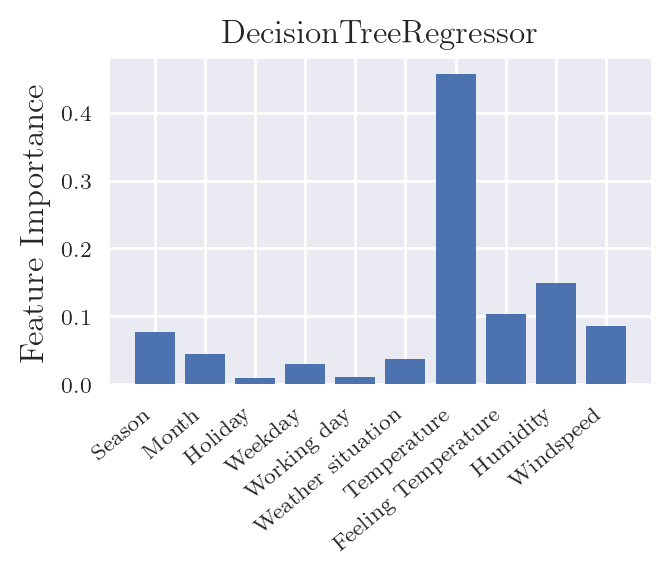
\includegraphics[width=0.55\textwidth]{w02_interpretable_models/figures/dt_bike_sharing.png}

    \end{frame}
    
    \begin{frame}{Risk Factors for Cervical Cancer (Classification)}
        
        \begin{itemize}
            \item Target: patient will get cancer or not?
            \item Reference: \lit{Fernandes et al. 2017}{https://link.springer.com/chapter/10.1007/978-3-319-58838-4_27}
            \item Exemplary features:
            \begin{itemize}
                \item Age in years
                \item Number of sexual partners
                \item First sexual intercourse (age in years)
                \item Number of pregnancies
                \item Smoking yes or no
                \item Smoking (in years)
                \item Hormonal contraceptives yes or no
                \item Hormonal contraceptives (in years)
                \item Intrauterine device yes or no (IUD)
            \end{itemize}
        \end{itemize}
        
    \end{frame}
	
	\begin{frame}{Logistic Regression on  Cancer (Classification)}
        
        \centering
        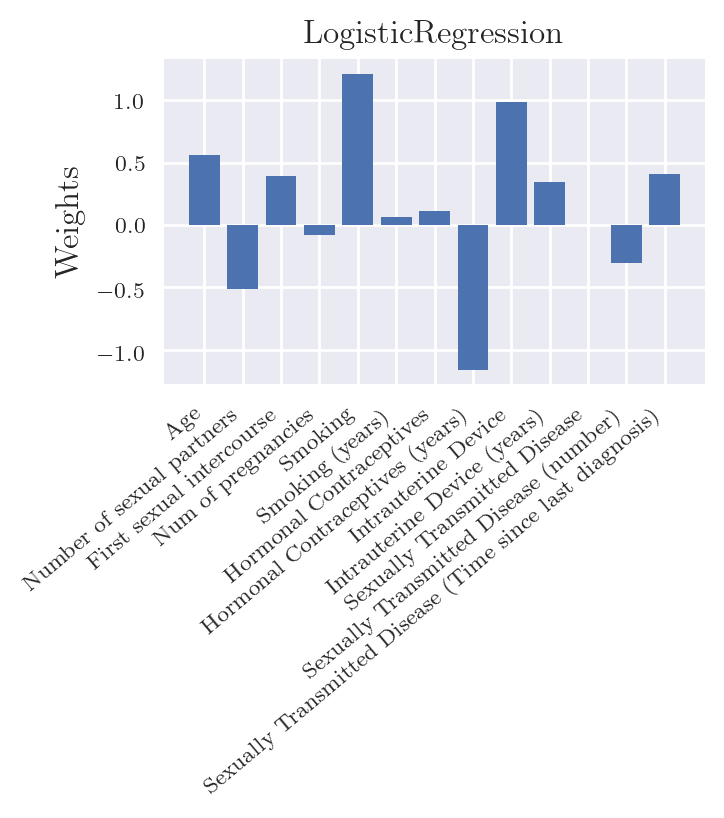
\includegraphics[width=0.55\textwidth]{w02_interpretable_models/figures/lin_cancer.png}
        
    \end{frame}
	
	\begin{frame}{Decision Tree on  Cancer (Classification)}
        
        \centering
        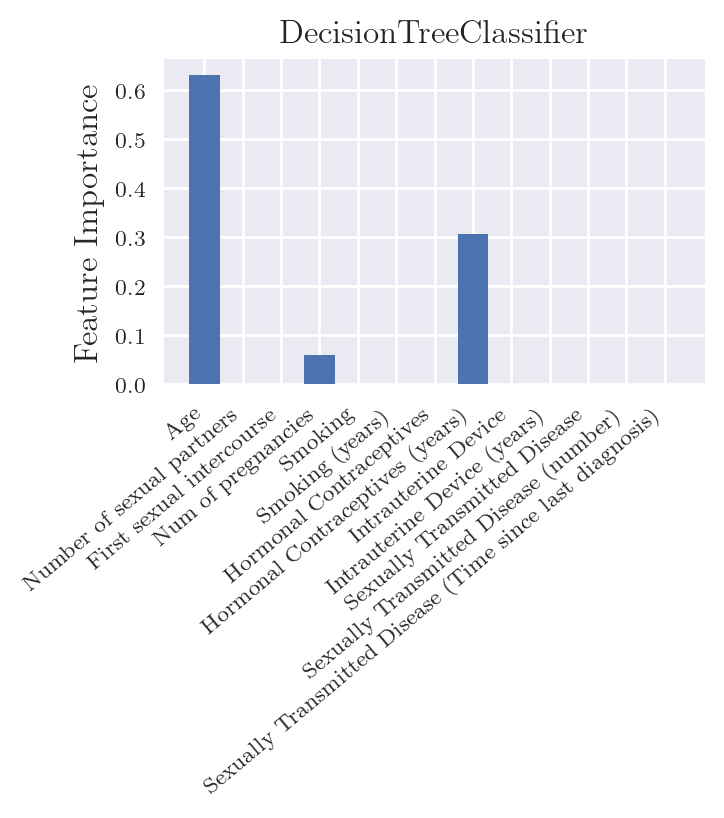
\includegraphics[width=0.55\textwidth]{w02_interpretable_models/figures/dt_cancer.png}
    \end{frame}
	
	\begin{frame}{Predictive Performance}
        
        \begin{itemize}
            \item Bike Rental (normalized MSE):
            \begin{itemize}
                \item Linear Regression: 0.0276
                \item Decision Tree: 0.0328
                \item GLM: 0.0244
            \end{itemize}
            \pause
            \medskip
            \item Cancer (Accuracy)
            \begin{itemize}
                \item Logistic Regression: 0.58
                \item Decision Tree: 0.62
            \end{itemize}
            \pause
            \smallskip
            \item[$\leadsto$] although easy to interpret, not really well-performing 
            \begin{itemize}
                \item Boosting: 0.79
            \end{itemize}
        \end{itemize}
        
    \end{frame}
	
\end{document}
